\subsubsection{\texttt{RF-7}: descarga de soluciones}
\label{subsec:rf7}

Tal como se introduce en los dos epígrafes anteriores, uno de los objetivos principales fijados para la evolución del proyecto es permitir a los estudiantes descargar las propuestas de solución adjuntadas por el profesorado a los ejercicios realizados siempre y cuando hayan sido publicadas por ellos.

Este requerimiento afecta a profesores y a estudiantes de forma diferente, por lo que da lugar a en dos requisitos según el rol:
\begin{itemize}
    \item El requisito \texttt{RF-7.1} establece que los estudiantes deben poder tener acceso a la descarga de la solución de un ejercicio siempre que exista solución y que haya sido publicada por los profesores.
    
    Para incorporar este punto, se ha aprovechado la implementación del requisito \texttt{RF-7.2}, introduciendo un control específico para usuarios con rol de estudiantes sobre la disponibilidad de la solución. En caso de que se den las condiciones adecuadas, se habilita un nuevo botón para la descarga de la solución y se lanza un aviso en la parte inferior del entorno de desarrollo, tal como ilustra la \referenciaFigura{fig:reqf7-1}.

    Al presionar el botón, aparece un cuadro de diálogo modal que informa al estudiante acerca de si tendrá la capacidad de editar posteriormente su ejercicio o si se marcará automáticamente como ``finalizado'' tras descargar la solución. Una vez el estudiante confirme que desee continuar, la solución se descargará y situará en un nuevo directorio llamado ``solution'' ubicado en el nivel inmediatamente inferior al del directorio padre del ejercicio activo.

    Adicionalmente, se han ampliado las capacidades del botón de refresco de la extensión y, en caso de que haya un ejercicio activo, la acción desencadenada por su utilización también verificará si la solución ha sido publicada desde la última vez que se descargó el ejercicio, favoreciendo la usabilidad de esta funcionalidad de modo que los estudiantes no tengan que desactivar y volver a acceder un ejercicio para comprobar si la solución ya es pública.
    \item El requisito \texttt{RF-7.2} determina que los profesores deben tener acceso a la solución que han adjuntado a sus propios ejercicios ---en caso de haberla---, descargándose junto con la plantilla y las propuestas de resolución parciales o finales de los estudiantes al activar un ejercicio desde la extensión.
    
    Para ejecutar la implementación de este requisito, se han tomado como ejemplo los métodos y procedimientos dispuestos tanto en servidor como en cliente para la descarga de la plantilla, reutilizando el código ---y previniendo la aparición de duplicidades--- para la implementación de esta capacidad. Como consecuencia, la solución se descarga en paralelo a la plantilla para los profesores independientemente de su estado de publicación.
\end{itemize}

\begin{figure}[ht]
    \centering
    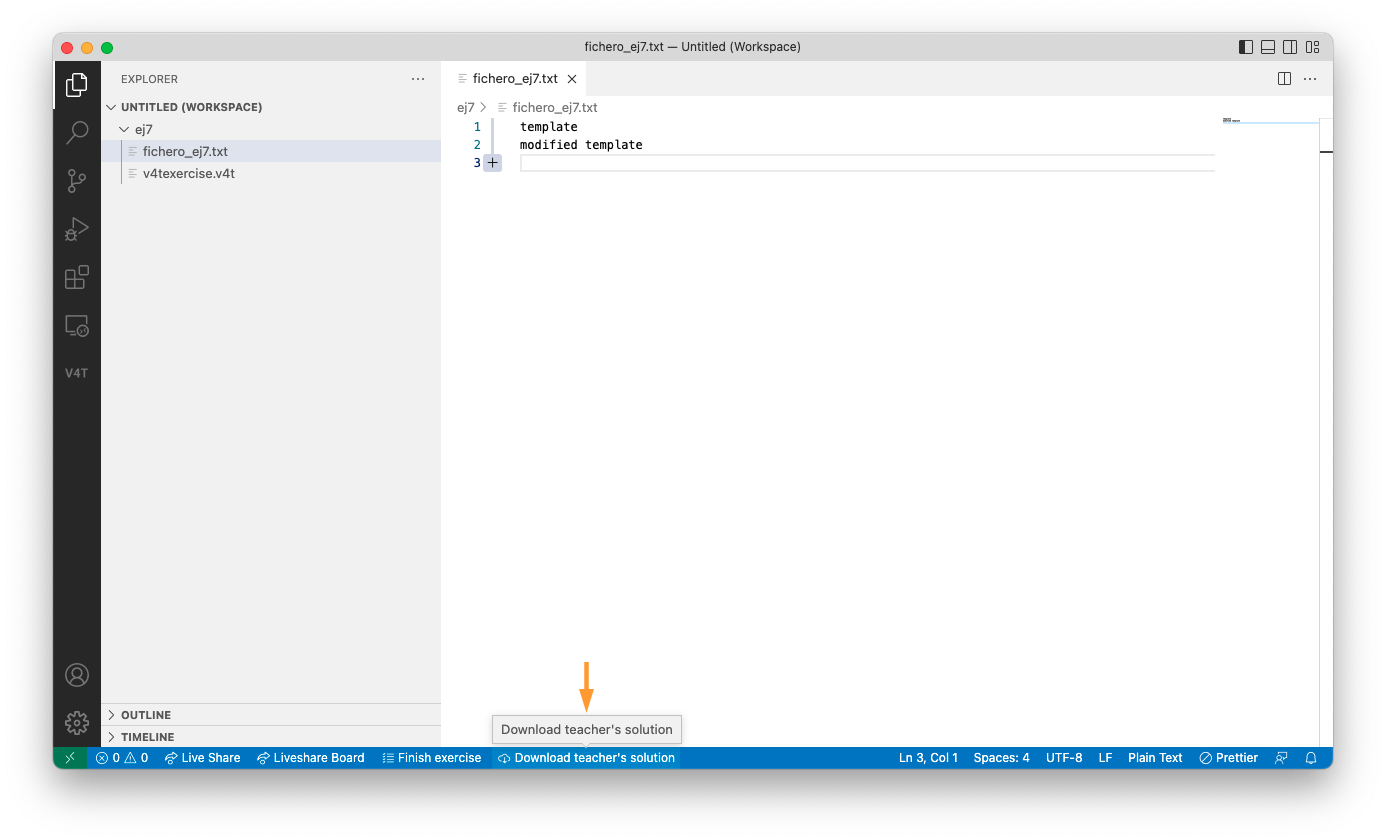
\includegraphics[width=\textwidth]{imagenes/utilizadas/4-3-implementacion/rf7-1.png}
    \caption{Captura de la extensión en la que se destaca el botón habilitado para la descarga de soluciones a ejercicios.}
    \label{fig:reqf7-1}
\end{figure}
